\documentclass[12pt]{article}
\usepackage[utf8]{inputenc}
\usepackage{float}
\usepackage{amsmath}

\usepackage[hmargin=3cm,vmargin=6.0cm]{geometry}
%\topmargin=0cm
\topmargin=-2cm
\addtolength{\textheight}{6.5cm}
\addtolength{\textwidth}{2.0cm}
%\setlength{\leftmargin}{-5cm}
\setlength{\oddsidemargin}{0.0cm}
\setlength{\evensidemargin}{0.0cm}

%misc libraries goes here
\usepackage{fitch}
\usepackage{tikz}
\usepackage{nicematrix}
\usepackage{amsmath}

\begin{document}

\section*{Student Information } 
%Write your full name and id number between the colon and newline
%Put one empty space character after colon and before newline
Full Name : Mithat Can Timurcan\\
Id Number :  2581064\\

% Write your answers below the section tags
\section*{Answer 1}
\begin{itemize}
 \item Let's look at our graph $G$. Since for every vertex, there's a path to all vertices, we can see that the graph is connected. Let's also write the degrees of all vertices:
 \begin{equation*}
  \begin{split}
   deg(a) = deg(b) = deg(f) = deg(k) = deg(m) = 2
  \end{split}
 \end{equation*}
 \begin{equation*}
  \begin{split}
   deg(c) = deg(d) = deg(e) = deg(g) = deg(h) = deg(i) = deg(j) = deg(l) = 4
  \end{split}
 \end{equation*}
\end{itemize}

\subsection*{a)}
\begin{itemize}
 \item By the Theorem 1 on the Section 10.5 of the textbook, since $G$ is connected and all of it's vertices have even degrees, we can say that there exists an Eulerian circuit.
 \item A sample circuit can be written as follows: $a-c-b-g-k-l-h-g-c-d-h-i-l-m-j-i-d-e-f-j-e-a$.
\end{itemize}
\subsection*{b)}
\begin{itemize}
 \item By the Theorem 2 on the Section 10.5 of the textbook, since our graph $G$ is connected, we only need to have 2 odd degreed vertices in order to have an Eulerian path which is not a circuit.
 \item Since all of our vertices have even degrees, we can see that there is no Eulerian path which is not a circuit.
\end{itemize}
\subsection*{c)}
\begin{itemize}
 \item A Hamilton Circuit is a circuit that traverses all vertexes (except the starting vertex) once. Although there's no easy way to conclude that there is no Hamilton circuit in our graph, according to the textbook (last paragraph of page 699), we can check 3 properties:
 \begin{itemize}
	\item A graph with a vertex of degree one cannot have a Hamilton circuit, because in a Hamilton circuit, each vertex
	is incident with two edges in the circuit. 
	\item If a vertex in the graph has degree two, then both edges that are incident with this vertex must be part of any Hamilton circuit.
	\item A Hamilton circuit cannot contain a smaller circuit within it.
 \end{itemize}
 \item However in our graph, the vertexes $a, b, f, k, m$ have degree of two. For the second property, the edges incident with those vertices must be included in our Hamilton circuit. When we consider those edges, we have a smaller circuit. We get a contradiction with the 3rd rule. Therefore, we can say thay there exists no Hamilton circuit in our graph $G$.
\end{itemize}
\subsection*{d)}
\begin{itemize}
 \item A Hamilton Path is a path that traverses all vertexes once. According to Ore's theorem, a simple graph has a Hamiltonian Path if for every pair of vertices
 in $G$ sum of their degrees is greater than $n-1$ where $n = |V|$. In our case, $n = 13$. There's no such pair that satisfy this condition. So, we can't conclude anything from Ore's Theorem. However, we can try to find a path ourselves. Such path can be: $a-c-b-g-k-l-m-j-f-e-d-h-i$.
\end{itemize}
\subsection*{e)}

\begin{figure}[H]
	\centering
	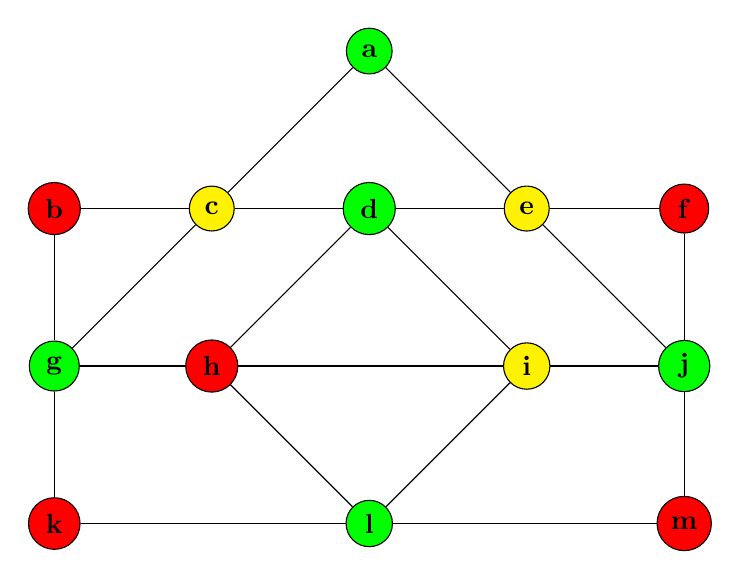
\begin{tikzpicture}

	\node[shape=circle,draw=black,fill=green] (a) at (4, 6)     {\textbf{a}};
	\node[shape=circle,draw=black,fill=red] (b) at (0, 4)     {\textbf{b}};
	\node[shape=circle,draw=black,fill=yellow] (c) at (2, 4)     {\textbf{c}};
	\node[shape=circle,draw=black,fill=green] (d) at (4, 4)     {\textbf{d}};
	\node[shape=circle,draw=black,fill=yellow] (e) at (6, 4)     {\textbf{e}};
	\node[shape=circle,draw=black,fill=red]  (f) at (8, 4)     {\textbf{f}};
	\node[shape=circle,draw=black,fill=green]  (g) at (0, 2)     {\textbf{g}};
	\node[shape=circle,draw=black,fill=red]  (h) at (2, 2)     {\textbf{h}};
	\node[shape=circle,draw=black,fill=yellow]  (i) at (6, 2)     {\textbf{i}};
	\node[shape=circle,draw=black,fill=green]  (j) at (8, 2)     {\textbf{j}};
	\node[shape=circle,draw=black,fill=red]  (k) at (0, 0)     {\textbf{k}};
	\node[shape=circle,draw=black,fill=green]  (l) at (4, 0)     {\textbf{l}};
	\node[shape=circle,draw=black,fill=red]  (m) at (8, 0)     {\textbf{m}};

	\path[-] (a) edge  node[left]  {} (c);
	\path[-] (b) edge  node[above] {} (c);
	\path[-] (c) edge  node[right] {} (d);
	\path[-] (d) edge  node[left]  {} (e);
	\path[-] (e) edge  node[right] {} (j);
	\path[-] (h) edge  node[right] {} (l);
	\path[-] (d) edge  node[right] {} (i);
	\path[-] (l) edge  node[right] {} (i);
	\path[-] (g) edge  node[below] {} (c);
	\path[-] (b) edge  node[below] {} (g);
	\path[-] (h) edge  node[below] {} (i);
	\path[-] (a) edge  node[right] {} (e);
	\path[-] (e) edge  node[right] {} (f);
	\path[-] (f) edge  node[right] {} (j);
	\path[-] (d) edge  node[right] {} (h);
	\path[-] (i) edge  node[below] {} (j);
	\path[-] (g) edge  node[below] {} (h);
	\path[-] (g) edge  node[below] {} (k);
	\path[-] (k) edge  node[below] {} (l);
	\path[-] (l) edge  node[below] {} (m);
    \path[-] (m) edge  node[right] {} (j);

	\end{tikzpicture}
	\caption{Coloring of the graph $G$.}
\end{figure}
\begin{itemize}
 \item From Figure 1. we can say that the chromatic number of this graph is $\chi(G)=3$.
 \item In 2-colorable graphs, there is no simple cycle such has an odd number of edges. A sample cycle $a-c-g-h-i-j-e-a$ has 7 edges, leading us to use at least 3 colors to color those vertices.
\end{itemize}
\subsection*{f)}
\begin{itemize}
 \item Since the chromatic number of our graph $G$ is $\chi(G) = 3 \neq 2$, we can say that it's not bipartite.
 \item We need to delete the edges forming an odd numbered cycle. Such edges will be $\{b, g\}, \ \{f, j\}$ and $\{h, i\}$.
 \item Now let's check our graph again, if it's 2-colorable, then we can say that it's bipartite:
 \begin{figure}[H]
	\centering
	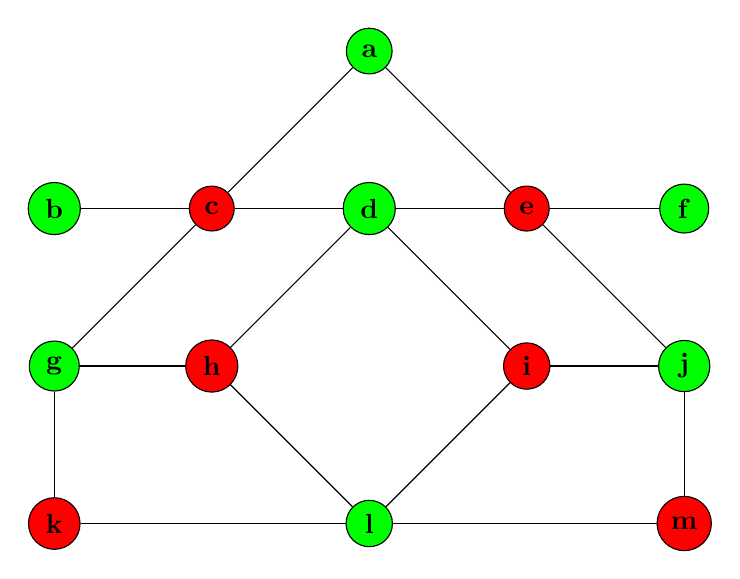
\begin{tikzpicture}

	\node[shape=circle,draw=black,fill=green] (a) at (4, 6)     {\textbf{a}};
	\node[shape=circle,draw=black,fill=green] (b) at (0, 4)     {\textbf{b}};
	\node[shape=circle,draw=black,fill=red] (c) at (2, 4)     {\textbf{c}};
	\node[shape=circle,draw=black,fill=green] (d) at (4, 4)     {\textbf{d}};
	\node[shape=circle,draw=black,fill=red] (e) at (6, 4)     {\textbf{e}};
	\node[shape=circle,draw=black,fill=green]  (f) at (8, 4)     {\textbf{f}};
	\node[shape=circle,draw=black,fill=green]  (g) at (0, 2)     {\textbf{g}};
	\node[shape=circle,draw=black,fill=red]  (h) at (2, 2)     {\textbf{h}};
	\node[shape=circle,draw=black,fill=red]  (i) at (6, 2)     {\textbf{i}};
	\node[shape=circle,draw=black,fill=green]  (j) at (8, 2)     {\textbf{j}};
	\node[shape=circle,draw=black,fill=red]  (k) at (0, 0)     {\textbf{k}};
	\node[shape=circle,draw=black,fill=green]  (l) at (4, 0)     {\textbf{l}};
	\node[shape=circle,draw=black,fill=red]  (m) at (8, 0)     {\textbf{m}};

	\path[-] (a) edge  node[left]  {} (c);
	\path[-] (b) edge  node[above] {} (c);
	\path[-] (c) edge  node[right] {} (d);
	\path[-] (d) edge  node[left]  {} (e);
	\path[-] (e) edge  node[right] {} (j);
	\path[-] (h) edge  node[right] {} (l);
	\path[-] (d) edge  node[right] {} (i);
	\path[-] (l) edge  node[right] {} (i);
	\path[-] (g) edge  node[below] {} (c);
	\path[-] (a) edge  node[right] {} (e);
	\path[-] (e) edge  node[right] {} (f);
	\path[-] (d) edge  node[right] {} (h);
	\path[-] (i) edge  node[below] {} (j);
	\path[-] (g) edge  node[below] {} (h);
	\path[-] (g) edge  node[below] {} (k);
	\path[-] (k) edge  node[below] {} (l);
	\path[-] (l) edge  node[below] {} (m);
    \path[-] (m) edge  node[right] {} (j);
	\end{tikzpicture}
	\caption{New coloring of the graph $G$.}
\end{figure}
\item Since we can now color it using only 2 colors, we can say that it's bipartite and therefore, the minimum number of edges that should be removed to make this graph bipartite is $3$.
\end{itemize}
\subsection*{g)}
\begin{itemize}
	\item No, there isn't any subgraphs that contain the complete graph with 4 vertices since our graph's chromatic number is $\chi(G) = 3$. Complete graphs are always $n$-colorable where $n$ denotes the number of vertices because all vertices are connected to each other.
	\item We can add an edge between the vertices $d$ and $l$ to obtain a subgraph that is complete.
	\begin{figure}[H]
		\centering
		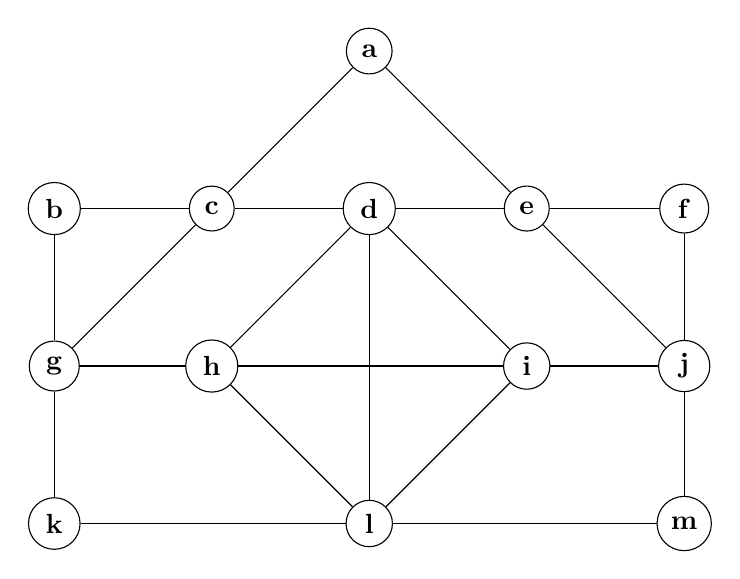
\begin{tikzpicture}
	
		\node[shape=circle,draw=black,fill=white] (a) at (4, 6)     {\textbf{a}};
		\node[shape=circle,draw=black,fill=white] (b) at (0, 4)     {\textbf{b}};
		\node[shape=circle,draw=black,fill=white] (c) at (2, 4)     {\textbf{c}};
		\node[shape=circle,draw=black,fill=white] (d) at (4, 4)     {\textbf{d}};
		\node[shape=circle,draw=black,fill=white] (e) at (6, 4)     {\textbf{e}};
		\node[shape=circle,draw=black,fill=white]  (f) at (8, 4)     {\textbf{f}};
		\node[shape=circle,draw=black,fill=white]  (g) at (0, 2)     {\textbf{g}};
		\node[shape=circle,draw=black,fill=white]  (h) at (2, 2)     {\textbf{h}};
		\node[shape=circle,draw=black,fill=white]  (i) at (6, 2)     {\textbf{i}};
		\node[shape=circle,draw=black,fill=white]  (j) at (8, 2)     {\textbf{j}};
		\node[shape=circle,draw=black,fill=white]  (k) at (0, 0)     {\textbf{k}};
		\node[shape=circle,draw=black,fill=white]  (l) at (4, 0)     {\textbf{l}};
		\node[shape=circle,draw=black,fill=white]  (m) at (8, 0)     {\textbf{m}};
	
		\path[-] (a) edge  node[left]  {} (c);
		\path[-] (b) edge  node[above] {} (c);
		\path[-] (c) edge  node[right] {} (d);
		\path[-] (d) edge  node[left]  {} (e);
		\path[-] (e) edge  node[right] {} (j);
		\path[-] (h) edge  node[right] {} (l);
		\path[-] (d) edge  node[right] {} (i);
		\path[-] (l) edge  node[right] {} (i);
		\path[-] (g) edge  node[below] {} (c);
		\path[-] (b) edge  node[below] {} (g);
		\path[-] (h) edge  node[below] {} (i);
		\path[-] (a) edge  node[right] {} (e);
		\path[-] (e) edge  node[right] {} (f);
		\path[-] (f) edge  node[right] {} (j);
		\path[-] (d) edge  node[right] {} (h);
		\path[-] (i) edge  node[below] {} (j);
		\path[-] (g) edge  node[below] {} (h);
		\path[-] (g) edge  node[below] {} (k);
		\path[-] (k) edge  node[below] {} (l);
		\path[-] (l) edge  node[below] {} (m);
		\path[-] (m) edge  node[right] {} (j);
		\path[-] (d) edge  node[right] {} (l);
	
		\end{tikzpicture}
		\caption{New graph $G'$ which has a complete graph with 4 vertices as a subgraph.}
	\end{figure}
\end{itemize}

\section*{Answer 2}
\begin{itemize}
 \item First of all, we need to check the graph invariants. If they're the same, we can continue.
 \begin{itemize}
 \item \textbf{Number of vertices:} 8 for graph $G$, 8 for graph $H$. They're the same.
 \item \textbf{Number of edges:} 16 for graph $G$, 16 for graph $H$. They're the same.
 \item \textbf{Degrees of vertices:} Every vertex in graph $G$ has the degree of 4, every vertex im graph $H$ also has the degree 4. They're the same.
 \end{itemize}
 \item Since the graph invariants are the same, now we need to find a bijective isomorphism function to map the graph $G$'s vertexes to graph $H$'s vertexes. From now on, let's denote this function as $f$.
 \item We should examine the cycles and try to preserve the edges, by doing so we get the following isomorphisim function:
 \begin{equation*}
	\begin{split}
		f(a) = a', \ f(b) = c', \ f(c) = e', \ f(d) = g' 
	\end{split}
   \end{equation*}
   \begin{equation*}
	\begin{split}
		f(e) = b', \ f(f) = h', \ f(g) = d', \ f(h) = f' 
	\end{split}
   \end{equation*}
   \item We now have a bijection between the vertex sets of G and H. Let's check the adjacency matrixes of $G$ and $H$:
   \begin{figure}[H]
	\centering
	$\begin{bNiceMatrix}[first-row,last-row,first-col,last-col]
		& a & b & c & d & e & f & g & h  \\
	a & 0 & 1 & 0 & 1 & 1 & 1 & 0 & 0 &  \\
	b & 1 & 0 & 1 & 0 & 1 & 0 & 1 & 0 &  \\
	c & 0 & 1 & 0 & 1 & 0 & 0 & 1 & 1 &  \\
	d & 1 & 0 & 1 & 0 & 0 & 1 & 0 & 1 &  \\
	e & 1 & 1 & 0 & 0 & 0 & 1 & 0 & 1 &  \\
	f & 1 & 0 & 0 & 1 & 1 & 0 & 1 & 0 &  \\
	g & 0 & 1 & 1 & 0 & 0 & 1 & 0 & 1 &  \\
	h & 0 & 0 & 1 & 1 & 1 & 0 & 1 & 0 &  \\
	\\
	\end{bNiceMatrix}$
	\caption{Adjacency matrix representation for graph $G$, $M_G$.}
	\end{figure}
	\begin{figure}[H]
		\centering
		$\begin{bNiceMatrix}[first-row,last-row,first-col,last-col]
			& a' & c' & e' & g' & b' & h' & d' & f'  \\
		a' & 0 & 1 & 0 & 1 & 1 & 1 & 0 & 0 &  \\
		c' & 1 & 0 & 1 & 0 & 1 & 0 & 1 & 0 &  \\
		e' & 0 & 1 & 0 & 1 & 0 & 0 & 1 & 1 &  \\
		g' & 1 & 0 & 1 & 0 & 0 & 1 & 0 & 1 &  \\
		b' & 1 & 1 & 0 & 0 & 0 & 1 & 0 & 1 &  \\
		h' & 1 & 0 & 0 & 1 & 1 & 0 & 1 & 0 &  \\
		d' & 0 & 1 & 1 & 0 & 0 & 1 & 0 & 1 &  \\
		f' & 0 & 0 & 1 & 1 & 1 & 0 & 1 & 0 &  \\
		\\
		\end{bNiceMatrix}$
		\caption{Adjacency matrix representation for graph $H$, $M_H$.}
	\end{figure}
	\item Since $M_G = M_H$, we can see that our isomorphism function $f$, preserves edges. Therefore, we've shown that graphs $G$ and $H$ are isomorphic.
\end{itemize}

\section*{Answer 3}
\subsection*{a)}
\begin{itemize}
	\item For odd number of vertices $(n=3,5,7, \cdots)$: The chromatic number is 3. This is because we can't color an odd cycle with just 2 colors without causing adjacent vertices to share the same color. For example, in a triangle, alternating colors will result in the first and last vertex (which are adjacent) being the same color if only two colors are used.
    \item For even number of vertices $(n=4,6, \cdots)$: The chromatic number is 2. This is because we can actually alternate between two colors around the cycle and return to the starting vertex with a different color than the one we started with.
    \item If a graph is 2-colorable, then we can say that it's bipartite. Therefore, we can say that for even number of vertices $C_n$ is bipartite. However, for odd number of vertices, $C_n$ is not bipartite.
\end{itemize}
\subsection*{b)}
\begin{itemize}
	\item For the $n$-dimensional cube graph $Q_n$, the graph will always be bipartite. We can show this by induction.
	\item \textbf{Base Case ($n = 1$):} $Q_1$ is a graph with two vertices connected by just one edge, we can clearly see that it's bipartite. We can set a partitioning such that no vertexes at those partitions connect each other.
	\item \textbf{Inductive Step ($n \geq 1$):}
	\begin{itemize}
		\item Assume that for some integer $k \geq 1$, $Q_k$ is bipartite. We need to show that $Q_{k+1}$ is also bipartite.
		\item We can form $Q_{k+1}$ by taking two copies of $Q_k$ and adding edges between corresponding vertices in these copies. In each copy, we're labeling the vertices such that they differ only by the $(k+1)$th bit.
		\item In $Q_k$, we can divide vertices into two sets based on the parity of the sum of their bits (even sum and odd sum) since $Q_k$ is bipartite by the inductive hypothesis.
		\item In $Q_{k+1}$, this property is preserved. One copy of $Q_k$ will have all vertices with an even sum of bits, and the other with an odd sum, considering the $(k+1)$th bit.
		\item Therefore, each edge in $Q_{k+1}$ either connects vertices with even bit sums to those with odd sums (within the same $Q_k$ copy) or connects corresponding vertices in different copies, which also have different parity sums.
		\item This shows that $Q_{k+1}$ is bipartite, completing our proof.
	\end{itemize}
	\item Since we've shown that cube graph $Q_n$ is always bipartite, we can say that it's 2-colorable and the graph chromatic number is equal to 2. $\chi(Q_n)=2$.
\end{itemize}
\section*{Answer 4}
\subsection*{a)}
\begin{itemize}
 \item We can use Kruskal's Algorithm to form a minimum spanning tree (MST).
 \item Let's write the steps of the algorithm:
 \begin{itemize}
  \item We are going to sort all the edges in non-decreasing order of their weights.
  \item We will pick the smallest edge (in terms of their weight) and check if it forms a simple circuit with the spanning tree formed so far. If it doesn't form a simple circuit, we can include this edge. Otherwise, we won't include that edge.
  \item We will repeat the 2nd step until there are $(V-1)$ edges in the spanning tree.
 \end{itemize}

\end{itemize}

\begin{table}[H]
	\small
	\centering
	\begin{tabular}{|c|c|c|}
	\hline
	Choice & Edge & Weight\\
	\hline
	1 & $\{a,b\}$ & 1\\
	2 & $\{c,e\}$ & 2\\
	3 & $\{c,f\}$ & 2\\
	4 & $\{a,d\}$ & 3\\
	5 & $\{b,c\}$ & 4 \\
	\hline
	\end{tabular}
	\end{table}
\subsection*{b)}
\begin{figure}[H]
	\centering
	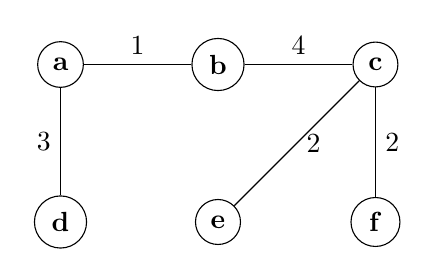
\begin{tikzpicture}

	\node[shape=circle,draw=black] (a) at (0, 4)     {\textbf{a}};
	\node[shape=circle,draw=black] (b) at (2, 4)     {\textbf{b}};
	\node[shape=circle,draw=black] (c) at (4, 4)     {\textbf{c}};
	\node[shape=circle,draw=black] (d) at (0, 2)     {\textbf{d}};
	\node[shape=circle,draw=black] (e) at (2, 2)     {\textbf{e}};
	\node[shape=circle,draw=black] (f) at (4, 2)     {\textbf{f}};

	\path[-] (a) edge  node[left]  {3} (d);
	\path[-] (a) edge  node[above] {1} (b);
	\path[-] (b) edge  node[above] {4} (c);
	\path[-] (c) edge  node[right] {2} (f);
	\path[-] (c) edge  node[right] {2} (e);

	\end{tikzpicture}
	\caption{Minimum Spanning Tree with Kruskal's algorithm for the given graph $G$}
\end{figure}
\subsection*{c)}
\begin{itemize}
 \item No, the minimum spanning tree we found is not the only one we can form. When we're picking the 2nd and 3rd edges while using Kruskal's Algorithm, we have more than one option. Such spanning trees can be also formed as follows:
\end{itemize}
\begin{figure}[H]
	\centering
	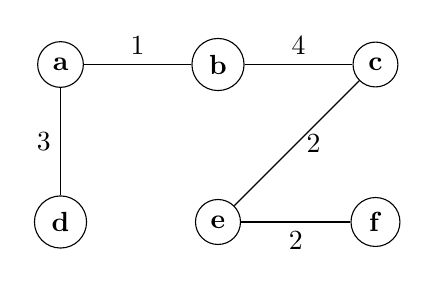
\begin{tikzpicture}

	\node[shape=circle,draw=black] (a) at (0, 4)     {\textbf{a}};
	\node[shape=circle,draw=black] (b) at (2, 4)     {\textbf{b}};
	\node[shape=circle,draw=black] (c) at (4, 4)     {\textbf{c}};
	\node[shape=circle,draw=black] (d) at (0, 2)     {\textbf{d}};
	\node[shape=circle,draw=black] (e) at (2, 2)     {\textbf{e}};
	\node[shape=circle,draw=black] (f) at (4, 2)     {\textbf{f}};

	\path[-] (a) edge  node[left]  {3} (d);
	\path[-] (a) edge  node[above] {1} (b);
	\path[-] (b) edge  node[above] {4} (c);
	\path[-] (e) edge  node[below] {2} (f);
	\path[-] (c) edge  node[right] {2} (e);

	\end{tikzpicture}
	\caption{2nd Minimum Spanning Tree with Kruskal's algorithm for the given graph $G$}
\end{figure}
\begin{figure}[H]
	\centering
	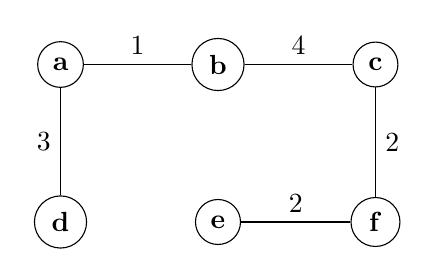
\begin{tikzpicture}

	\node[shape=circle,draw=black] (a) at (0, 4)     {\textbf{a}};
	\node[shape=circle,draw=black] (b) at (2, 4)     {\textbf{b}};
	\node[shape=circle,draw=black] (c) at (4, 4)     {\textbf{c}};
	\node[shape=circle,draw=black] (d) at (0, 2)     {\textbf{d}};
	\node[shape=circle,draw=black] (e) at (2, 2)     {\textbf{e}};
	\node[shape=circle,draw=black] (f) at (4, 2)     {\textbf{f}};

	\path[-] (a) edge  node[left]  {3} (d);
	\path[-] (a) edge  node[above] {1} (b);
	\path[-] (b) edge  node[above] {4} (c);
	\path[-] (c) edge  node[right] {2} (f);
	\path[-] (e) edge  node[above] {2} (f);

	\end{tikzpicture}
	\caption{3rd Minimum Spanning Tree with Kruskal's algorithm for the given graph $G$}
\end{figure}


\section*{Answer 5}
\subsection*{a)}
\begin{itemize}
 \item We can use mathematical induction on the tree's height $h$ to show that a full binary tree with $n$ vertices has $\frac{n+1}{2}$ leaf vertices.
 \item \textbf{Base Case ($h = 0$):}
 \begin{itemize}
  \item When the tree's height is 0, it only has 1 vertex which is also the leaf vertex. Since $\frac{1+1}{2} = 1$ leaf vertex, the property is satisfied when the tree's height is 0.
 \end{itemize}
 \item \textbf{Inductive Step ($h \geq 0$):}
 \begin{itemize}
  \item Assume that for a full binary tree of height $h$ with $n$ vertices, the property is satisfied. By the inductive hypothesis, the tree has $\frac{n+1}{2}$ leaf vertices.
  \item We need to prove the statement for the height $h+1$. In order to create a tree with height $h+1$, we add two children to one of the leaf vertices. Now we have $n+2$ total vertices.
  \item The original leaf vertex is now an branch vertex, and the new leaves are the newly added children. The original leaf adds 2 new leaves but we need to subtract the original leaf, so the number of leaves in the tree of height $h+1$ is $\frac{n+1}{2} + 2 - 1 = \frac{n+1}{2} + 1$. Let's calculate the number of leaf vertices with our formula, using $n + 2$ vertices:
  \begin{equation*}
   \begin{split}
    \dfrac{(n+2)+1}{2} = \dfrac{n+1}{2} + 1 \ \text{leaf vertices}
   \end{split}
  \end{equation*}
  \item Since we got the same result, we can say that the property is also satisfied when the height is $h+1$.
 \end{itemize}
 \item Therefore, we've shown that a full binary tree with n vertices has $\frac{n+1}{2}$ leaf vertices.
\end{itemize}


\subsection*{b)}
\begin{itemize}
	\item Let's denote the tree with $n$ vertices as $T_n$. The chromatic number of a tree will always be equal to 2. $\chi(T_n) = 2$.
	\item This property holds for every integer $n$ since trees are acyclic (containing no cycles) and connected graphs. We can always start from some vertex and color it with a specific color. Then, as we move away from that vertex along the edges, we will always alternate between the two colors for each level of the tree.
	\item Trees are also always bipartite graphs, meaning that we can set two partitions such that no vertices are not connected with each other in each partition. We can color the vertices in one partition same color, and for the other partition we can use another color, leading us having only 2 colors to color a tree.
\end{itemize}

\subsection*{c)}
\begin{itemize}
	\item To find the upper bound of a tree, we need to achieve the maximum height with the minimum number of nodes. In order to achieve this, we can add m nodes (since the tree will be full) to one child at each level while incrementing the height of the tree. We get the following tree:
	\begin{figure}[H]
		\centering
		\begin{tikzpicture}

		\coordinate (D1) at (3.5,2);
		\coordinate (D2) at (2.75,2);
		\coordinate (D3) at (4.25,2);
		\coordinate (D4) at (1,-0.5);
		\coordinate (D5) at (1,-1.25);
		\coordinate (D6) at (1,-2);
		\coordinate (D7) at (1.25,0);
		\coordinate (D8) at (1.5,0);
		\coordinate (D9) at (1.75,0);
		\coordinate (D10) at (1.25,-4.5);
		\coordinate (D11) at (1.5,-4.5);
		\coordinate (D12) at (1.75,-4.5);
		\foreach \dot in {D1,D2,D3,D4,D5,D6,D7,D8,D9,D10,D11,D12}
			\fill (\dot) circle (0.03);
	
		\node[shape=circle,draw=black] (a) at (1, 2)     {};
		\node[shape=circle,draw=black] (b) at (3, 4)     {};
		\node[shape=circle,draw=black] (c) at (6, 2)     {};
		\node[shape=circle,draw=black] (d) at (0, 0)     {};
		\node[shape=circle,draw=black] (g) at (0.75, 0)     {};
		\node[shape=circle,draw=black] (h) at (2.25, 0)     {};
		\node[shape=circle,draw=black] (x) at (3, 0)     {};
		\node[shape=circle,draw=black] (e) at (2, 2)     {};
		\node[shape=circle,draw=black] (f) at (5, 2)     {};


		\node[shape=circle,draw=black] (t) at (1, -2.5)     {};
		\node[shape=circle,draw=black] (m) at (0, -4.5)     {};
		\node[shape=circle,draw=black] (l) at (0.75,-4.5)     {};
		\node[shape=circle,draw=black] (k) at (2.25, -4.5)     {};
		\node[shape=circle,draw=black] (y) at (3, -4.5)     {};
	
		\path[-] (a) edge  node[left]  {} (d);
		\path[-] (a) edge  node[left]  {} (g);
		\path[-] (a) edge  node[left]  {} (h);
		\path[-] (a) edge  node[left]  {} (x);
		\path[-] (a) edge  node[above] {} (b);
		\path[-] (b) edge  node[above] {} (c);
		\path[-] (b) edge  node[above] {} (e);
		\path[-] (b) edge  node[above] {} (f);
	
		\path[-] (t) edge  node[left]  {} (m);
		\path[-] (t) edge  node[left]  {} (k);
		\path[-] (t) edge  node[left]  {} (l);
		\path[-] (t) edge  node[left]  {} (y);
		\end{tikzpicture}
		\caption{Full $m$-ary tree with $n$ nodes and height $h$.}
	\end{figure}
	\item Every level except the first level has $m$ nodes. Calculating the total number of nodes, we get $mh+1=n$. This equation is the minimum number of nodes to form a full $m$-ary tree with height $h$.
	\begin{equation*}
		\begin{split}
			mh + 1 \leq n \\
			h \leq \dfrac{n-1}{m}
		\end{split}
	\end{equation*}
	\item Therefore we can say that $\frac{n-1}{m}$ is the upper bound for height of a full $m$-ary tree.
\end{itemize}

\end{document}
